\documentclass{standalone}
\usepackage{tikz,tikz-3dplot} 

\usetikzlibrary{calc,intersections}

\begin{document}
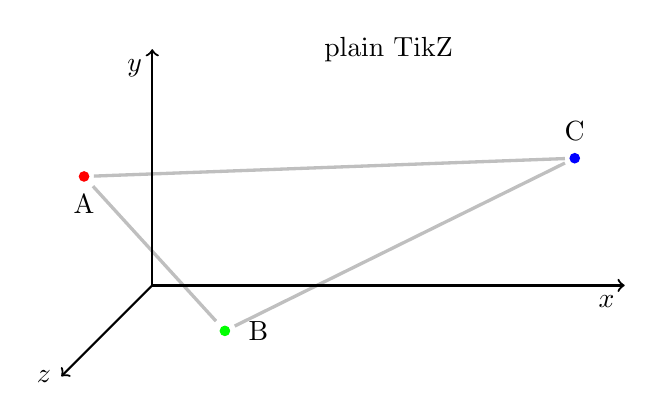
\begin{tikzpicture}[scale=3]

	\node[] (title) at (1, 1, 0) {plain TikZ};
    
    \draw[thick,->,black] (0,0,0) -- (2,0,0) node[anchor=north east]{$x$};
    \draw[thick,->] (0,0,0) -- (0,1,0) node[anchor=north east]{$y$};
    \draw[thick,->] (0,0,0) -- (0,0,1) node[anchor=east]{$z$};
    
    \filldraw[red] (0,0.75,0.75) circle (0.02cm) node (A) {} node[anchor=north,fill=white,yshift=-0.1cm, text=black] {A};
    \filldraw[green] (0.5,0,0.5) circle (0.02cm) node (B) {} node[anchor=west,fill=white,xshift=5pt, text=black] {B};
    \filldraw[blue] (1.75,0.5, -0.1) circle (0.02cm) node (C) {} node[anchor=south,fill=white,yshift=0.1cm, text=black] {C};
    
     \draw[name path=diagonal,very thick, opacity=0.25] (A) -- (B);
     \draw[name path=diagonal,very thick, opacity=0.25] (B) -- (C);
     \draw[name path=diagonal,very thick, opacity=0.25] (C) -- (A);
     
     
    
\end{tikzpicture}


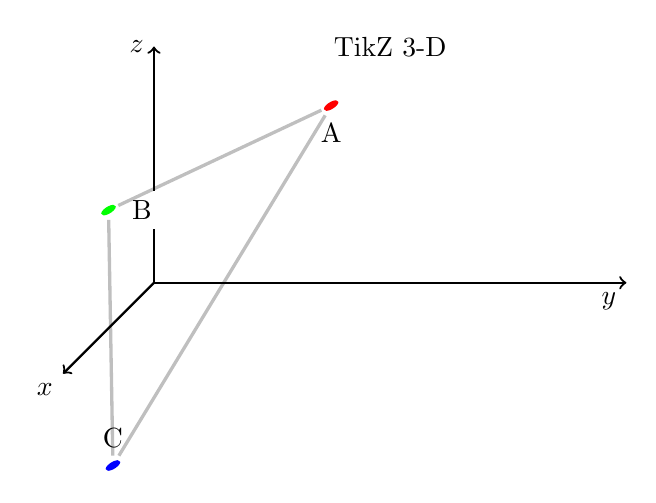
\begin{tikzpicture}[scale=3,cm={-1,-1,1,0,(0,0)},x=3.85mm,z=-1cm]
	\node[] (title) at (0, 1, 1) {TikZ 3-D};
	
    \draw[thick,->,black] (0,0,0) -- (1,0,0) node[anchor=north east]{$x$};
    \draw[thick,->] (0,0,0) -- (0,2,0) node[anchor=north east]{$y$};
    \draw[thick,->] (0,0,0) -- (0,0,1) node[anchor=east]{$z$};
    
    \filldraw[red] (0,0.75,0.75) circle (0.02cm) node (A) {} node[anchor=north,fill=white,yshift=-0.1cm, text=black] {A};
    \filldraw[green] (0.5,0,0.5) circle (0.02cm) node (B) {} node[anchor=west,fill=white,xshift=5pt, text=black] {B};
    \filldraw[blue] (1.75,0.5, -0.1) circle (0.02cm) node (C) {} node[anchor=south,fill=white,yshift=0.1cm, text=black] {C};
    
    \draw[name path=diagonal,very thick, opacity=0.25] (A) -- (B);
    \draw[name path=diagonal,very thick, opacity=0.25] (B) -- (C);
    \draw[name path=diagonal,very thick, opacity=0.25] (C) -- (A);
    

    
\end{tikzpicture}



\end{document}
